\chapter{Evaluation}
\label{ch:evaluation}

In this chapter we present the evaluation of the methods proposed in the previous part, chapter~\ref{ch:reducing}. We should mention that we did not include in all the results in this chapter to prevent cluttering. Further experimentations can be found in appendix. First we present individual results for each of the methods. We also give details about the methodology and the parameter choices. The final comparison is illustrated at the end of this subsection using an error \textit{vs.} time representation.

The methods were compared in this section on the top 3 largest data sets as number of points $N$.

\section{Evaluation setup}
\label{sec:setup}

The evaluation was done in terms of two metrics: accuracy and speed. An additional and more subjective criterion is to judge a method by visualizing low dimensional representations of various data sets. We provided 2D plots of the projected data where suitable.

The data sets selected for testing are listed in table~\ref{tab:datasets}. We note that the used data vary both as number of samples~$N$ and as dimensionality~$D$. Even if we concentrate on large amounts of data, we need small data sets to assess the performance of new models. The methods' speed was tested on the large data sets (\texttt{usps}, \texttt{magic} and \texttt{mnist}). However, this diversity of the data sets' size and complexity made it difficult to find the optimal selection of parameters. We are aware that there is ``no free lunch'' in accurately solving widely different problems with a fixed model. When concentrating on a single task it is often advised to include prior knowledge into the model. Also it is easier to make minor tweaks of the parameters to boost the performance.

\begin{table}%`
  \centering
    \begin{tabular}{l l c c c} \toprule
	Data set name&Abbrevation&$N$&$D$&$C$\\ 
	\midrule
	Balance scale&\texttt{balance}&$625$&$4$&$3$\\ 
	Ecoli&\texttt{ecoli}&$336$&$7$&$8$\\ 
% 	&\texttt{fruit}&$59$&$3$&$3$\\ 
	Glass identification&\texttt{glass}&$214$&$9$&$6$\\ 
	Ionosphere&\texttt{ionosphere}&$351$&$33$&$2$\\ 
	Iris&\texttt{iris}&$150$&$4$&$3$\\ 
	Landsat satellite&\texttt{landsat}&$6435$&$36$&$6$\\ 
	MAGIC Gamma telescope&\texttt{magic}&$19020$&$10$&$2$\\ 
	MNIST digits&\texttt{mnist}&$70000$&$784$&$10$\\ 
% 	&\texttt{olivetti}&$400$&$4096$&$40$\\ 
	Pima Indians diabetes&\texttt{pima}&$768$&$8$&$2$\\ 
	Image segmentation&\texttt{segment}&$2310$&$18$&$7$\\ 
	SPECTF heart&\texttt{spectf}&$267$&$44$&$2$\\ 
	Blood transfusion&\texttt{transfusion}&$748$&$4$&$2$\\ 
	USPS digits&\texttt{usps}&$11000$&$256$&$10$\\ 
	Wine&\texttt{wine}&$178$&$13$&$3$\\ 
	Yeast&\texttt{yeast}&$1484$&$8$&$10$\\  
      \bottomrule
    \end{tabular}
    \caption{\small \small This table presents the characteristics of the data sets used: number of samples $N$, dimensionality of the data $D$ and number of classes $C$. The two digits data sets \texttt{mnist} and \texttt{usps} were downloaded from the following URL \protect\url{http://cs.nyu.edu/~roweis/data.html}. All the others data sets are available in the UCI repository \protect\url{http://archive.ics.uci.edu/ml/datasets.html}.}
    \label{tab:datasets}
\end{table}

For evaluation we used $70\%$ of the data set for training and the rest of $30\%$ was kept for testing. We made exceptions for two data sets: \texttt{landsat} and \texttt{mnist}. These are commonly already split in training and testing sets.

The methods we test are: sub-sampling (SS; section~\ref{sec:sub-sampling}), mini-batches (MB; section~\ref{sec:mini-batches}), stochastic learning (SL; section~\ref{sec:stochastic-learning}). For stochastic learning we included the two approximated methods: the fast kernel density estimation idea (SL-KDE; section~\ref{sec:approximate}) and compact support version of NCA (SL-CS; section~\ref{sec:exact-computations}). Each method has particular parameters that we discuss in its corresponding subsection.

There are some common parameters for all the methods. These choices are related to NCA implementation and, for convenience, we remind them here. We experimented with three optimization methods: gradient ascent with ``bold driver'' heuristic, conjugate gradients and variants of stochastic gradient ascent with early stopping. For initialization we used the techniques described in subsection~\ref{subsec:initialization}: random initialization, PCA, LDA or RCA. At test time, we did classification using $1$-NN or using an NCA based function as in subsection~\ref{subsec:doing-classification}. However, we usually present scores using both classification rules.

The experiments were carried in \textsc{Matlab} and most of the implementations are the authors' own work. There are some exceptions however. We used Carl E. Rasmussen's \texttt{minimize.m} for conjugate gradient optimization. The RCA implementation was downloaded from \url{http://www.openu.ac.il/home/shental/}. Also we used functions from Iain Murray's \textsc{Matlab} toolbox. 

\section{Baseline}
\label{sec:baseline} 

We started by implementing the standard NCA algorithm (appendix \ref{app:code-nca-obj}). This consists the main baseline against which we compare new models.  
For our first series of experiments, we tried to replicate the work in the original article \citep{goldberger2004}. We encountered some difficulties since no information about their implementation was provided in the paper. Our results are presented in table \ref{table:eval-baseline}. We randomly initialized the matrix $\AB$ and optimized it using conjugate gradients. The scores are averaged over 40 runs. We note that the results are similar to those of \citet{goldberger2004}. 

\begin{table}
  \centering\begin{tabular}{lrcccc}
  \toprule
	  &     & Train score  & \multicolumn{2}{c}{Test scores} & Baseline \\
  \cmidrule(r){3-3} \cmidrule(r){4-5} \cmidrule(r){6-6}
  Data set & $d$ & $f(\AB)$ & $1$-NN & NCA & Eucl. \\
  \midrule
    \texttt{balance}&$2$&$92.86 \pm 0.47$&$90.78 \pm 0.53$&$90.61 \pm 0.55$&\\ 
		    &$D=4$&$95.36 \pm 0.38$&$93.40 \pm 0.47$&$93.04 \pm 0.51$&$76.18$\\ 
    \midrule
    \texttt{ionosphere}&$2$&$98.31 \pm 0.14$&$79.86 \pm 0.75$&$79.74 \pm 0.78$&\\ 
		       &$D=33$&$72.07 \pm 0.71$&$86.22 \pm 0.64$&$72.87 \pm 0.71$&$85.38$\\ 
    \midrule
    \texttt{iris}&$2$&$99.38 \pm 0.11$&$94.94 \pm 0.39$&$94.72 \pm 0.39$&\\ 
		 &$D=4$&$99.48 \pm 0.10$&$95.10 \pm 0.44$&$95.15 \pm 0.44$&$95.53$\\
    \midrule
    \texttt{wine}&$2$&$99.15 \pm 0.14$&$92.4 \pm 1.0$&$92.4 \pm 1.0$&\\ 
		 &$D=13$&$98.95 \pm 0.15$&$95.36 \pm 0.51$&$95.36 \pm 0.51$&$74.53$\\ 
  \bottomrule
  \end{tabular}
  \caption{\small Accuracy of standard NCA on four small data sets. Scores are averaged over 40 runs. The second column presents the dimensionality~$d$ the data set is reduced to. The last column shows the leave one out cross validation performance on the data set using Euclidean metric.}
  \label{table:eval-baseline}
\end{table}

% We used as a baseline a standard NCA implementation . 
% This allowed us to have a baseline to compare the new models against, table \ref{table:eval-baseline}.
% We started testing NCA on small data sets.  This can also be viewed as a replication of the work in the original article \citet{goldberger2004}. The authors did not provide us with any information about their implementation. For our first series of experiments, we used random initialization and we optimized the function using conjugate gradients. The results are averaged over 40 runs. We also considered the score obtained in the original space. We computed this using leave one out cross validation using the Euclidean metric. The results are quite similar to those presented in the original paper.  
% 
% Also for comparison we also offer scores from applying PCA, LDA and RCA followed by $1$-NN.

However, in order to achieve a robust implementation of NCA we had to carry out additional experiments. The learnt lessons were summarized in section~\ref{sec:practical-notes}. We will further see the influence of the implementation tricks in the next part (section~\ref{sec:method-comparison}). Results were shown in section~\ref{sec:practical-notes} and are also attached at the end of the thesis, appendix~\ref{app:results}:
\begin{itemize}
 \item Tables~\ref{table:comp-opts-1} and~\ref{table:comp-opts-2} compare two the optimization methods: conjugate gradients and gradient ascent with ``bold driver'' heuristic. We observe that the two methods give close scores on most of data sets. 
 \item Figures~\ref{fig:iris-init}, \ref{fig:balance-init} and~\ref{fig:ecoli-init} illustrate the initialization effect on three data sets: \texttt{iris}, \texttt{balance} and \texttt{ecoli}. RCA seems to be the best option for initialization and we used it in most of our comparisons. However, random projection can also be sometimes surprisingly good as we see in figure~\ref{fig:iris-init-2}. 
\end{itemize}

\section{Mini-batches methods}
\label{sec:method-comparison}

  We tested the methods on \texttt{usps}, \texttt{magic}, and \texttt{mnist}. We chosen to reduce the dimensionality to $d=5$. The decision is partially motivated by the fact NCA is very effective for reducing the data dimensionality to small values, somewhere around $5$ to $15$. A more principled approach would have been to develop of model choosing algorithm: start with a projection to $d=2$ dimensions and then increase the number of dimensions until the score stops improving. This can be illustrated for \texttt{landasat} data set.

  \begin{figure}
   \centering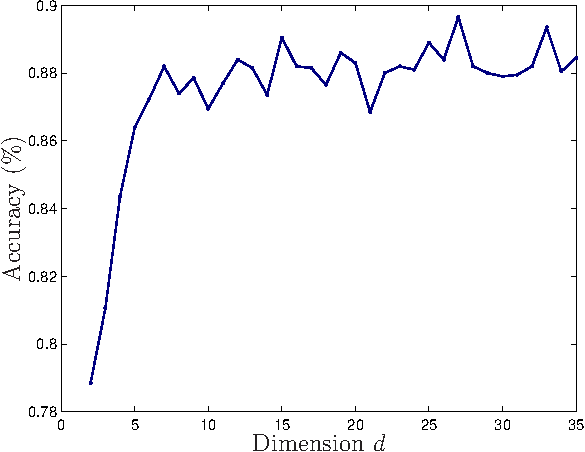
\includegraphics[width=0.6\textwidth]{images/landsat-evolution}
   \caption{Evolution of test accuracy as dimensionality increases. We see that NCA operates well in low dimensions. This approach can be used for selecting an optimal dimension to which we project the data.}
   \label{fig:landsat-evolution}
  \end{figure}


  \subsection{Sub-sampling}
  \label{subsec:eval-sub-sampling}

    For sub-sampling (SS) we trained NCA on a subset of $n=3000$ samples of the original data. We used conjugate gradients for optimization and RCA linear transformation for initialization. As previously mentioned in section \ref{sec:sub-sampling} the sub-sampled data has a thinner distribution than the original data which helps the method to obtain good scores at training. But the test performance is hindered because we do not use the true distribution. This is especially evident for the digits data \texttt{usps} and \texttt{mnist} (table \ref{tab:ss}). 
    \begin{table}
    	\centering
    	\begin{tabular}{lccc}
    	\toprule
    	Data set & Train & $1$-NN & NCA \\
    	\cmidrule(r){2-2}\cmidrule(r){3-3}\cmidrule(r){4-4} 
    	 \texttt{usps}&$99.112 \pm 0.099$&$89.30 \pm 0.18$&$89.41 \pm 0.16$\\
    	 \texttt{magic}&$82.71 \pm 0.41$&$79.25 \pm 0.45$&$80.22 \pm 0.72$\\
    	 \texttt{mnist}&$96.867$&$82.130$&$82.470$\\
    	 \bottomrule
    	\end{tabular}
	\label{tab:ss}
	\caption{Accuracy scores of sub-sampling method on three large data sets. We used RCA for initialization and CGs for optimization. We used a subset of $n=3000$ data points for training and the whole data set for testing.}
    \end{table}

    \subsection{Mini-batches}
    \label{subsec:eval-mini-batches}

    We trained NCA using gradient ascent on mini-batches as described in section~\ref{sec:mini-batches}. For the learning rate, we used an update rule of the form $\frac{\eta}{t+t_0}$. We fixed $\eta=1$ and tuned the other free parameter $t_0$ using cross validation across an exponential scale from $0.1$ to $1000$. After that, a finer tuning was done on a linear scale around the best value of $t_0$. We used $5\%$ of the training set for cross validation to monitor the accuracy score at each iteration. If the performance on the cross validation set does not increase for $25$ iterations, we stop the learning process and return to the previously best parameter.

    To get significant gradients we used large mini-batches $n=2000$. The points in a batch are selected via recursive projection clustering (RPC) algorithm. The clustering was done in the low dimensional space, after projecting the points with the current linear transformation matrix~$\AB$.
    The results obtained by mini-batches method can be found in table \ref{tab:mb}. 

    \begin{table}
        	\centering
        	\begin{tabular}{lccc}
        	\toprule
        	Data set & Train & $1$-NN & NCA \\
        	\cmidrule(r){2-2}\cmidrule(r){3-3}\cmidrule(r){4-4} 
        	 \texttt{usps}&$92.00 \pm 0.43$&$91.26 \pm 0.17$&$92.37 \pm 0.17$\\
        	 \texttt{magic}&$80.04 \pm 0.48$&$79.14 \pm 0.52$&$79.8 \pm 1.1$\\
        	 \texttt{mnist}&$87.47 \pm 0.49$&$87.52 \pm 0.36$&$89.88 \pm 0.25$\\
        	 \bottomrule
        	\end{tabular}
		\label{tab:mb}
		\caption{Accuracy scores of the mini-batches method on three large data sets. We used RCA for initialization and the mini-batches for clustered in the low-dimensional space using RPC. The size of a mini-batch was of maximum $n=2000$ data points.}
    \end{table}

    \subsection{Stochastic learning}
    \label{subsec:eval-stochastic-learning}

    This method was trained using a similar algorithm as before. We used the same parameters and early stopping. We considered $n=50$ neighbours to look at for each iteration and computed their contributions with respect to the whole data set. 

    Besides the results on the large data sets (table \ref{tab:sl-2}), we also present the performance of this method when used for small data sets (table \ref{tab:sl-1}). We mostly observe similar results as the baseline NCA. The most important remark is that the classification done using NCA objective function is better than $1$-NN classification. This observation also applies for the large data sets results. More results for this method are in appendix.

    \begin{table}
      \centering\begin{tabular}{lrccc}
      \toprule
	      &     & Train score  & \multicolumn{2}{c}{Test scores}\\
      \cmidrule(r){3-3} \cmidrule(r){4-5}
      Data set & $d$ & $f(A)$ & $1$-NN & NCA \\
      \midrule
	\texttt{balance}&$2$&$88.35 \pm 0.83$&$87.37 \pm 0.49$&$90.45 \pm 0.38$\\  
	&$D=4$&$94.70 \pm 0.87$&$95.32 \pm 0.34$&$96.14 \pm 0.29$\\ 
	\midrule
	\texttt{ionosphere}&$2$&$89.0 \pm 1.7$&$85.71 \pm 0.94$&$87.08 \pm 0.95$\\
	&$D=33$&$92.6 \pm 1.5$&$84.72 \pm 0.57$&$84.34 \pm 0.59$\\ 
	\midrule
	\texttt{iris}&$2$&$96.41 \pm 0.94$&$96.33 \pm 0.57$&$97.00 \pm 0.46$\\ 
	&$D=4$&$97.5 \pm 1.3$&$95.67 \pm 0.71$&$96.11 \pm 0.66$\\ 
	\midrule
	\texttt{wine}&$2$&$98.80 \pm 0.70$&$97.22 \pm 0.65$&$97.50 \pm 0.49$\\ 
	&$D=13$&$99.25 \pm 0.62$&$96.85 \pm 0.41$&$96.85 \pm 0.41$\\ 
      \bottomrule
      \end{tabular}
      \label{tab:sl-1}
      \caption{Stochastic learning results on small data sets. We used RCA for initialization. The scores are averaged after 20 iterations.}
    \end{table}

        \begin{table}
            	\centering
            	\begin{tabular}{lccc}
            	\toprule
            	Data set & Train & $1$-NN & NCA \\
            	\cmidrule(r){2-2}\cmidrule(r){3-3}\cmidrule(r){4-4} 
            	\texttt{usps}&$90.23  \pm 0.50$&$90.68 \pm 0.22$&$92.64 \pm 0.17$\\
            	\texttt{magic}&$78.39 \pm 0.25$&$79.76 \pm 0.13$&$84.49 \pm 0.12$\\
            	\texttt{mnist}&$85.97 \pm 0.37$&$86.07 \pm 0.43$&$89.35 \pm 0.39$\\
            	 \bottomrule
            	\end{tabular}
		\label{tab:sl-2}
		\caption{Accuracy scores of stochastic learning method on three large data sets. We used RCA for initialization. At each iteration we consider $n=50$ data points.}
        \end{table}

    \subsection{Comparison}
    \label{subsec:eval-comparison}

    To easily compare the 3 presented methods, we provide time-accuracy plots on the large data sets. We did not compute time for smaller data sets, since the classical NCA was usually fast enough. We also included in the plots the method based on the compact support kernels; we discuss its individual scores in the next subsection. 

    The differences in time varied strongly for the 4 methods so we had to use a logarithmic scale on the time. For each method we had also plotted its covariance matrix, but because of the logarithmic axis this looks deformed. In the plot the best methods are placed in the top left corner. 

    We note that the performance and the time spent varies quite heavily even for the same method. The number of iterations it takes for a method to converge is quite varied. There is a certain trade-off between time and accuracy, especially for the digits data sets. The stochastic learning and the mini batches seem to behave similarly. We could not also run the classic NCA, because of its cost. However, \citet{singh2010} did also experiment on \texttt{mnist} and she reported error of about $9\%$ for $d=5$.

      \begin{figure}
		\centering
		\subfigure[\texttt{usps}]{\label{fig:usps}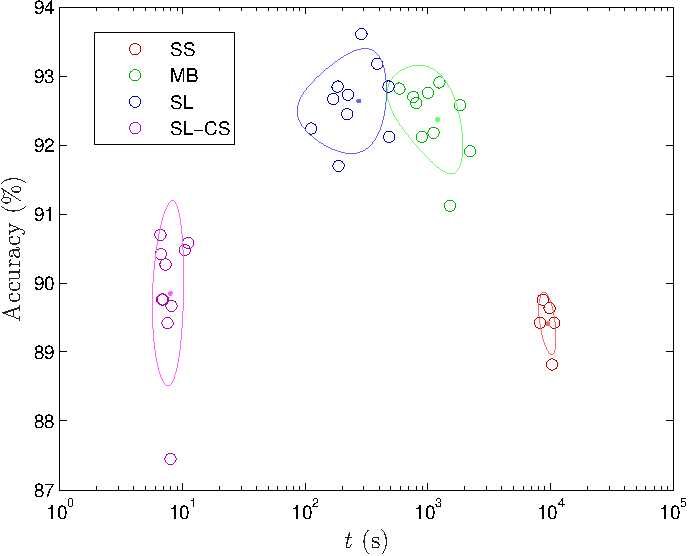
\includegraphics[width=0.61\textwidth]{images/usps-acc-time}}
		\subfigure[\texttt{magic}]{\label{fig:magic}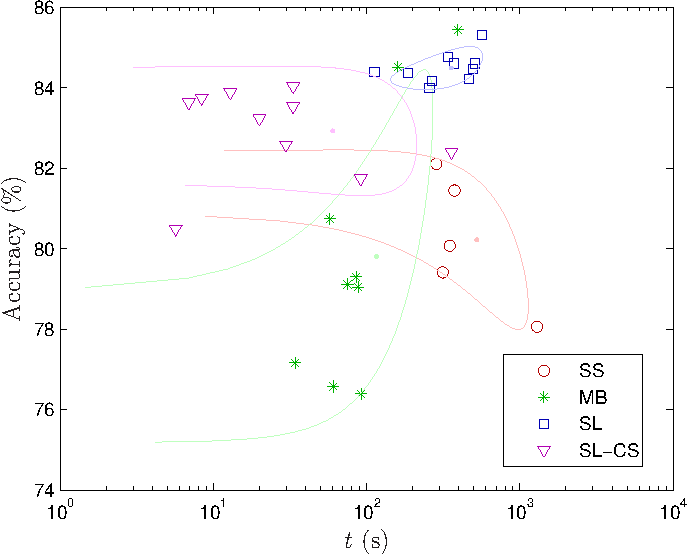
\includegraphics[width=0.61\textwidth]{images/magic-acc-time}}
		\subfigure[\texttt{mnist}]{\label{fig:mnist}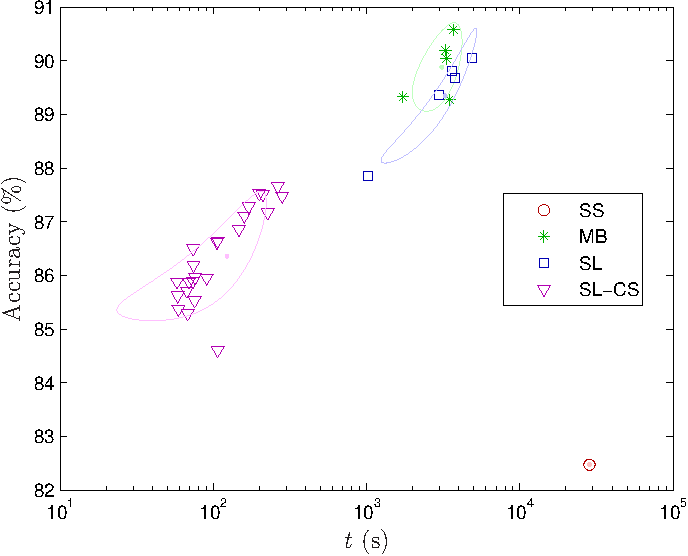
\includegraphics[width=0.61\textwidth]{images/mnist-acc-time}}
		\caption{\small Time \textsl{vs.} accuracy plots on larger data sets.}
		\label{fig:time-accuracy}
      \end{figure}


\section{Approximate computations}
\label{sec:eval-nca-approx}

Although the following methods can be applied on classic NCA, we tested them in conjunction with the stochastic learning procedure to further boost the speed of the method. In fact, we think that there is no worry to prefer the stochastic learning against the classical procedure.

\subsection{NCA with $k$-d trees}
\label{subsec:eval-nca-k-d-trees}

For the class-conditional density estimation we used a similar algorithm to that described in section \ref{sec:approximate}. Our implementation of $k$-d trees was done in \texttt{MATLAB} and it was pretty slow for this reason. The lack of vectorization when recursively computing the objective function and the gradient made the code slower than in the classical version. We also experimented with kernel density code written in C and mex-ed in \texttt{MATLAB}. From our experience we think that such an approach would be suitable and it would provide speed-ups. Doing simple kernel density estimation with a C written code is even faster than doing it in \texttt{MATLAB}. Unfortunately, the short time did not permit us to finish this implementation. However, we can demonstrate that  NCA with $k$-d trees achieves good results even if we discard a large number of the points. Table show results for this method on the three large data sets. We also present how the accuracy and the average number of prunings depends on the maximum error imposed. 

\subsection{NCA with compact support kernels}
\label{subsec:eval-nca-cs}

\begin{figure}
	\centering
	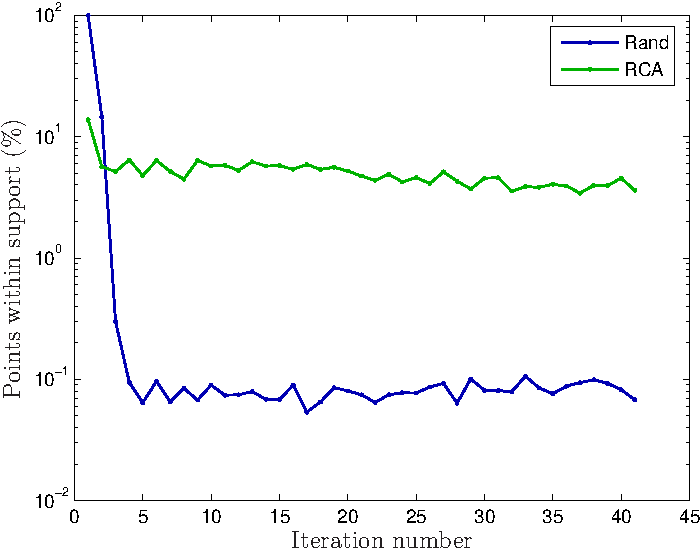
\includegraphics[width=0.6\textwidth]{images/nca-cs-nnzs}
\end{figure}

\begin{table}
            	\centering
            	\begin{tabular}{lccc}
            	\toprule
            	Data set & Train & $1$-NN & NCA \\
            	\cmidrule(r){2-2}\cmidrule(r){3-3}\cmidrule(r){4-4} 
\texttt{usps}&$85.16 \pm 0.33$&$87.02 \pm 0.44$&$89.85 \pm 0.30$\\ 
  \midrule
\texttt{magic}&$76.92 \pm 0.56$&$79.09 \pm 0.42$&$82.92 \pm 0.36$\\ 
  \midrule
\texttt{mnist}&$80.55 \pm 0.28$&$81.96 \pm 0.26$&$86.36 \pm 0.18$\\ 
  \bottomrule
  \end{tabular}
\end{table}

The compact support version of NCA was easy to implement and it is very fast as we already saw in section \ref{subsec:eval-comparison}. Usually only a small fraction of the points is inspected. In figure, we see how this fraction evolves with the learning process. In the first iterations there might be larger number of points, but soon this drops off and stabilizes. It might be tempting to start with all the points very close together to ensure that no point is outside the compact support of any other point. This approach has however two drawbacks. Since all the points are in the support of all the other points it means the first iteration will be quadratic in the number of the points. In fact, the first iteration can be easily as expensive as the whole learning process. A second issues is that the gradients will be very large and might ``throw away'' points out of the existing support. More reliable is an initialization with the linear transformation such as RCA. This provides a more stable evolution. We also see that the final projection looks better in the second case.

Results that demonstrate performance in terms of accuracy on small data sets are attached in appendix. The comparison in there is against the classical NCA and the extended version of NCA with compact support kernels and background distribution. The results on the large data set are available in table. 

\section{Recommendations}
\label{sec:eval-recommendations}

When dealing with a large data set, we suggest to first try NCA CS with stochastic learning. This method has the advantage of being easy to implement and very fast even for large data sets. However, the speed does come at a cost. We note a slight decrease in accuracy for most experimentations. Nonetheless, this is very good to get an idea of how well NCA can perform on a given data set. If one is pleased with the score, it can use the classic NCA with stochastic learning and hope to get an improvement of a couple of percentages in accuracy.